\section*{Aufgabe 3}

\subsection*{a)}
Im ersten Schritt mögliche Aktionen:
$ \left\{ \Out{a}{} \right\} $ \\


Mit $ \Pro{B} \CCSDef a.\Pro{A}$ ist zu zeigen: \\
$ \Relabel*{ \Res{\left( a.\Pro{A} | \Out{b}{}.\Pro{A} \right)}{a}}{a/b} \CCSTrans{\Out{a}{}}
 \Relabel*{ \Res{\left( a.\Pro{A} | \Pro{A} \right)}{a}}{a/b} $ \\


Beweis:


\begin{figure}[h]
\centering
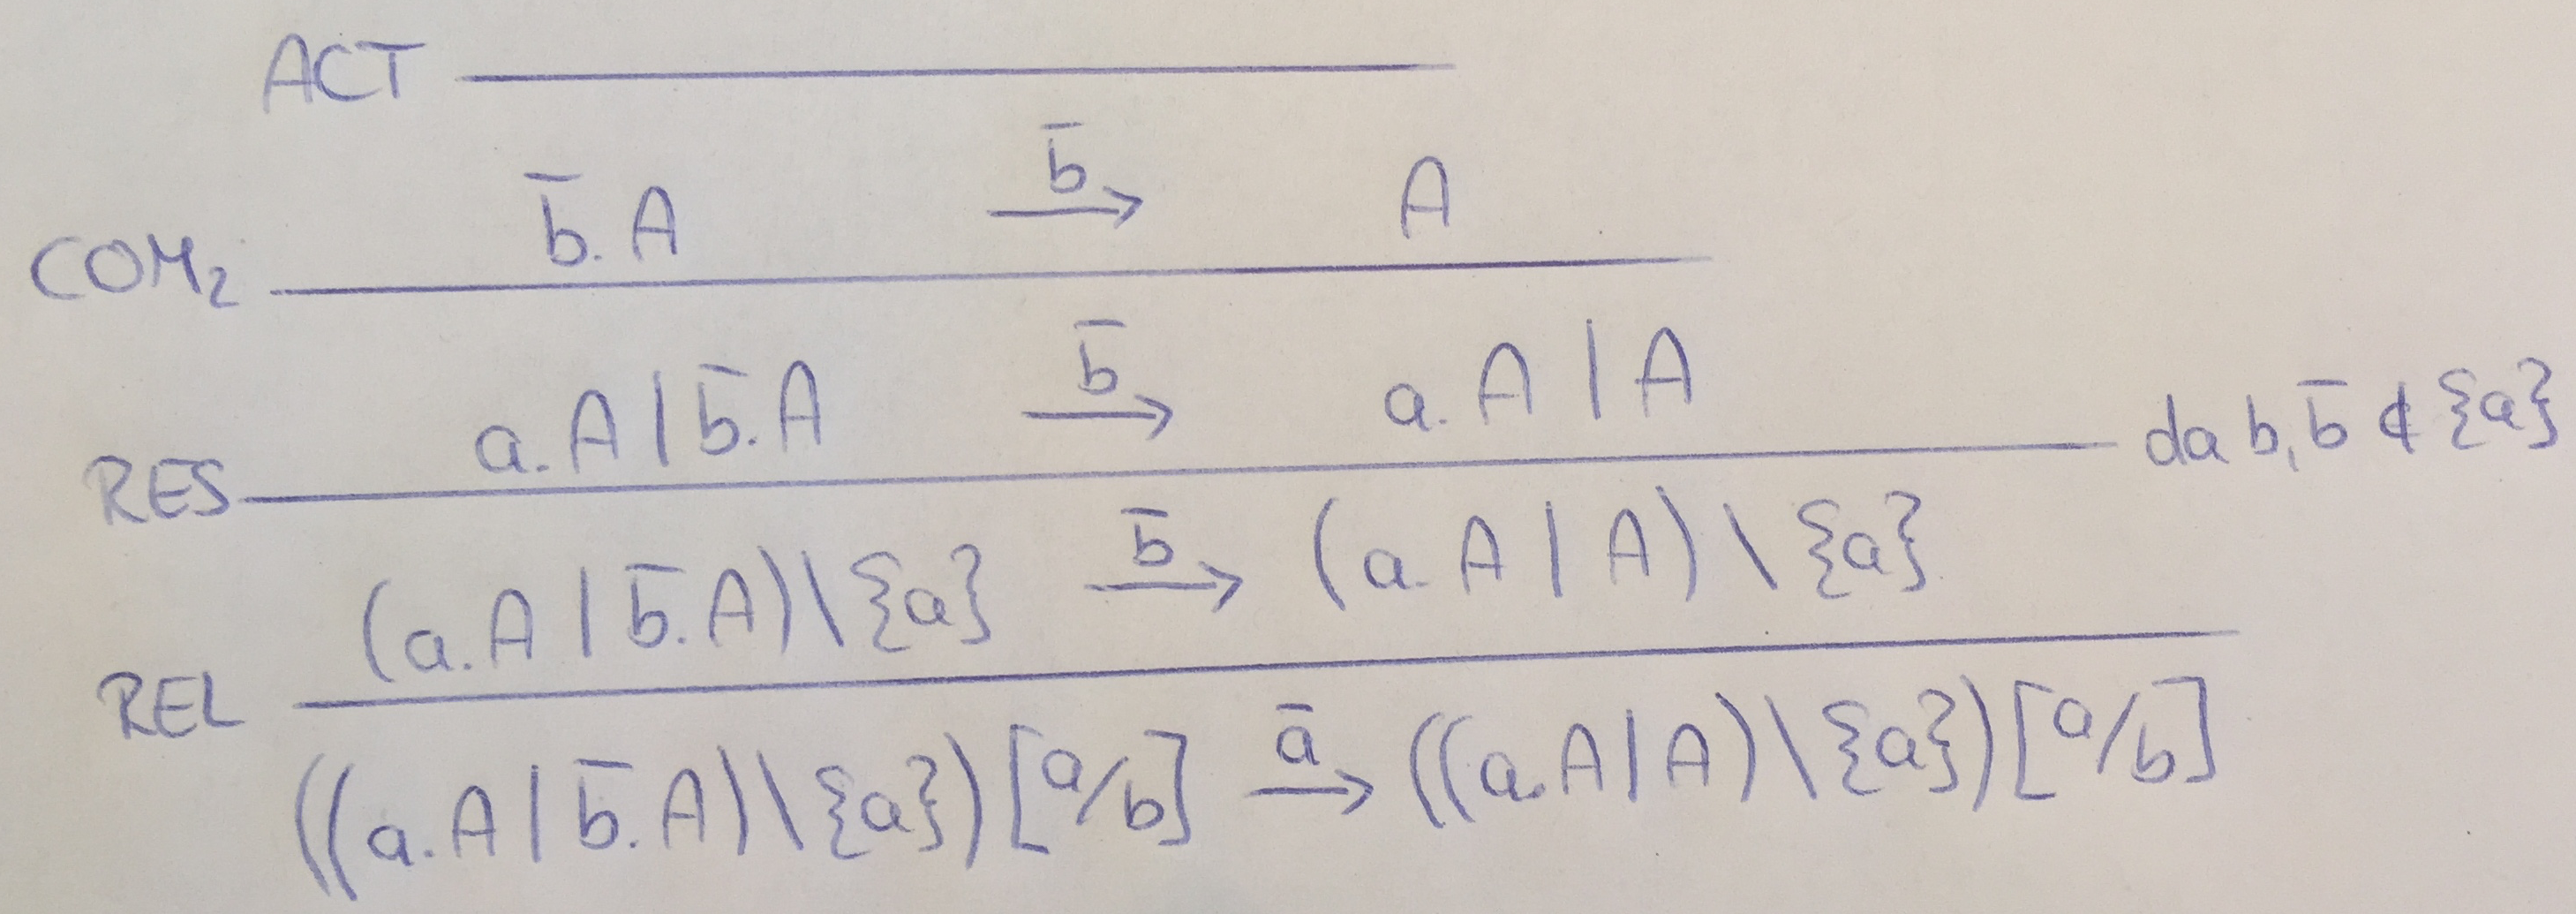
\includegraphics[width=\textwidth]{aufgabe3-a.png}
\end{figure}

\subsection*{b)}
Es sind keine Aktionen möglich: $ \emptyset $ \\

\subsection*{c)}
Im ersten Schritt mögliche Aktionen:
$ \left\{ \tau \right\} $ \\


Mit $ \Pro{B} \CCSDef a.\Pro{A}$ ist zu zeigen: \\
$ \Res*{ a.\Pro{A} | \Relabel*{\Out{b}{}.\Pro{A}}{a/b}}{a} \CCSTrans{\tau}
\Res*{\Pro{A} | \Relabel*{\Pro{A}}{a/b}}{a}$ \\

Beweis:\\


\begin{figure}[h]
\centering
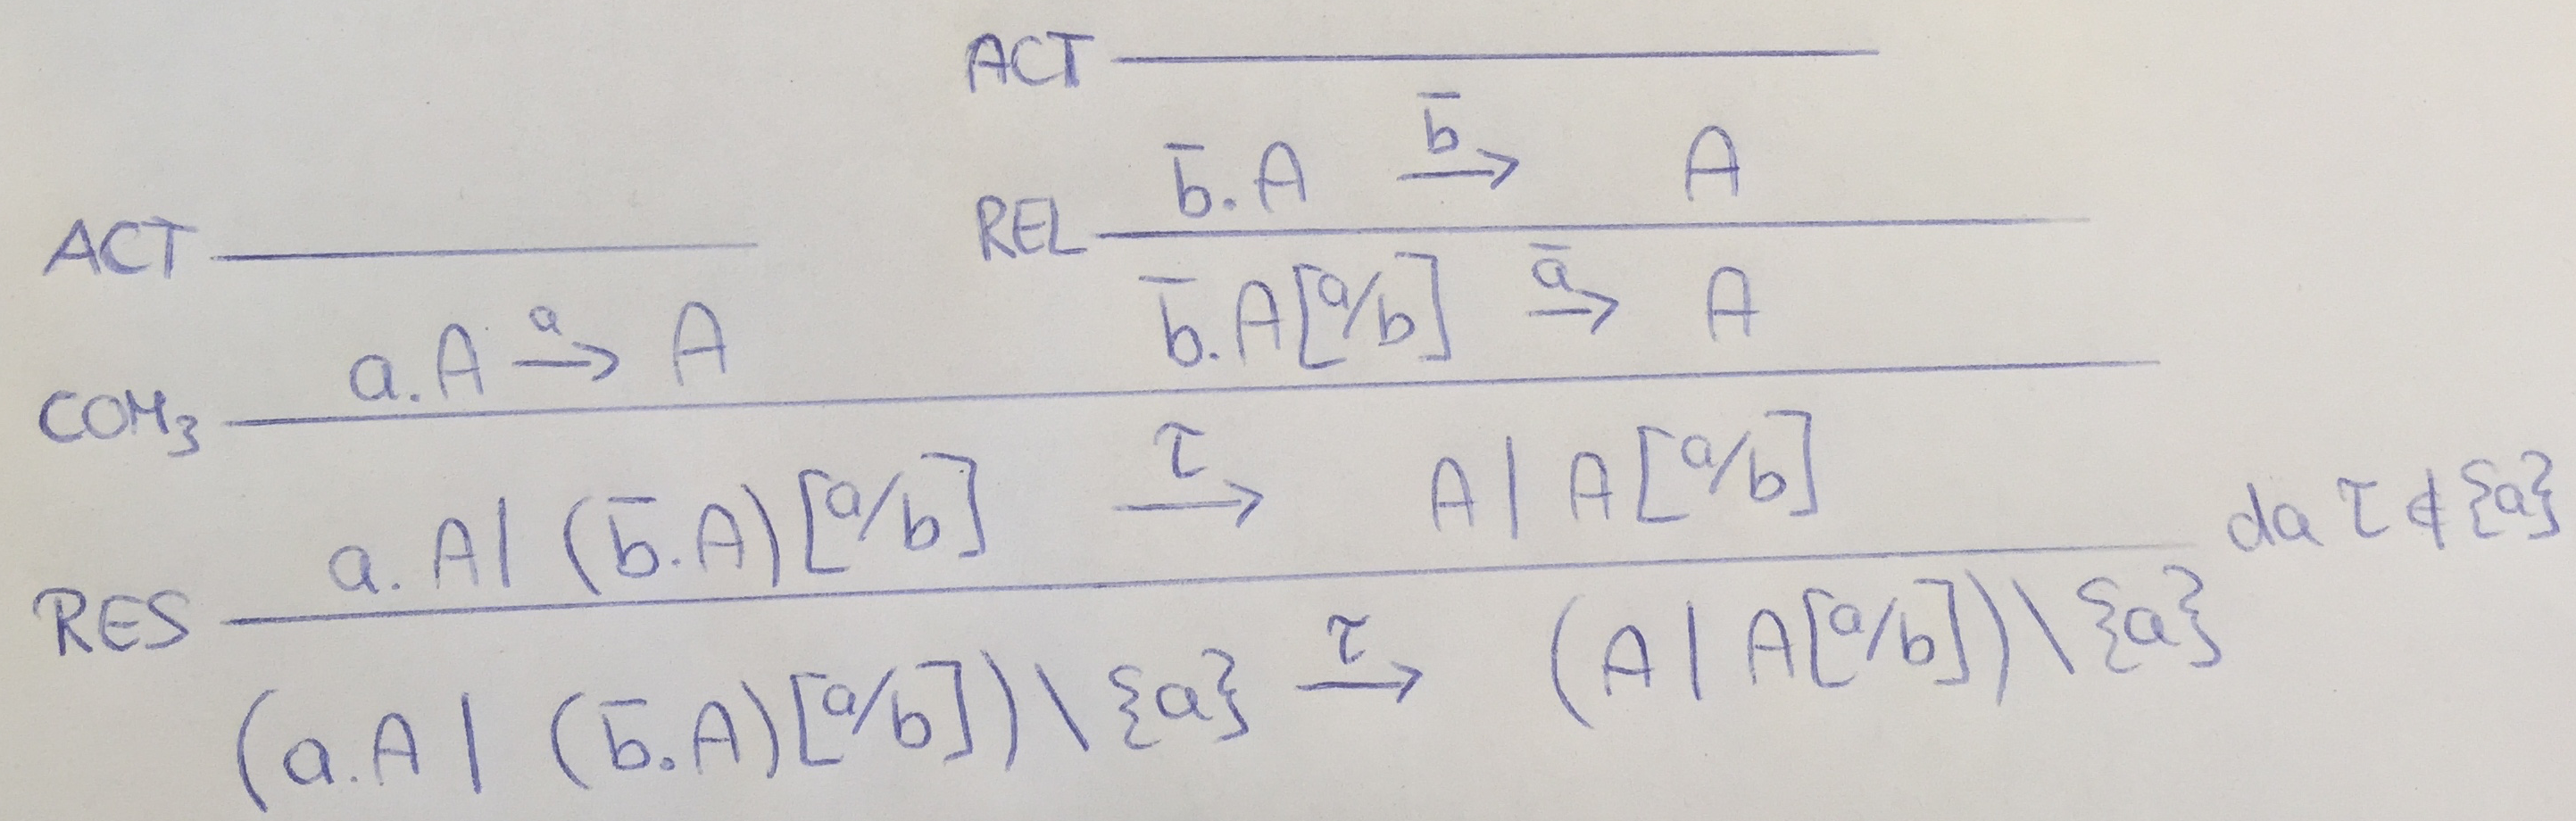
\includegraphics[width=\textwidth]{aufgabe3-c.png}
\end{figure}
